\documentclass[12pt,a4paper]{article}

\usepackage[left=1.5cm, right=1.5cm, top=1cm, bottom=2cm]{geometry}

\usepackage[T1]{fontenc}
\usepackage[utf8]{inputenc}
\usepackage{upgreek}
\usepackage{polski}
\usepackage[polish]{babel}

\usepackage{listings}
\usepackage{array}
\usepackage{amsmath}
\usepackage{mathtools}
\usepackage{caption}
\usepackage{tocloft}
\usepackage{tabularx}
\usepackage{xcolor,colortbl}
\usepackage{hhline}
\usepackage{wrapfig}
\usepackage{enumitem}
\usepackage{graphicx}
\usepackage{titlesec}
\usepackage{subfig}
\usepackage{pdflscape}
\usepackage{qtree}
\usepackage{hyperref}

\author{Mateusz Szwed \\Piotr Dulęba}
\title{
\includegraphics[width=0.5\linewidth]{graphics/logo_AGH} \\ \vspace{30pt}
Wydział Informatyki, Elektroniki i Telekomunikacji \\ \vspace{20pt}
\textbf{Prosty mikrokontroler w logice programowalnej -\\sprawozdanie z laboratorium.} \\ \vspace{20pt} Rok akademicki 2018/2019 \\ \vspace{30pt}}
\date{05.03.2019}
\begin{document}
	\maketitle
	\newpage
	\section{Pisanie własnego programu (zadanie 3.5)}
	W pliku \texttt{mem\_init\_start.coe} zapisaliśmy wymagane instrukcje, które dawały następujące rezultaty:
	
	\subsection{Wpisanie liczby 0x05 do komórki o adresie 13.}
	
	\begin{table}[!ht]
		\centering
		\begin{tabular}{l|l|l|l}
		Opis                                          & OPCODE & MNEMONIC & BYTE CODE \\ \hline
		wpisuje liczbę 0x05 do rejestru R0            & 85     & MOV 0x05 & 10000101  \\
		wpisuje wartość spod rejestru R0 pod adres 13 & ED     & STR 0, 0xD & 11101101 
		\end{tabular}
	\end{table}
	
	Rezultat:
	
	\begin{figure}[!ht]
		\centering
		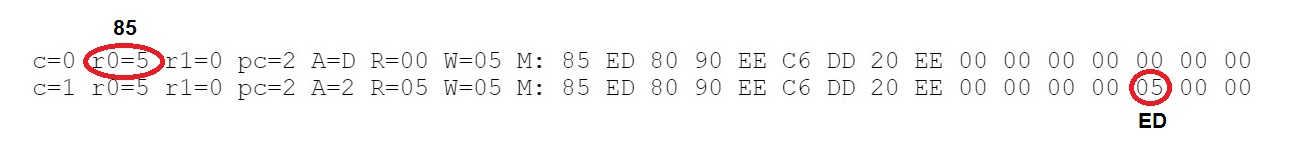
\includegraphics[width=1\linewidth]{graphics/log1}
	\end{figure}

	\subsection{Wyczyścić zawartość rejestrów R0 i R1, wpisując do nich 0.}
	
	\begin{table}[!ht]
		\centering
		\begin{tabular}{l|l|l|l}
		Opis                               & OPCODE & MNEMONIC & BYTE CODE \\ \hline
		wpisuje liczbę 0x00 do rejestru R0 & 80     & MOV 0x0  & 10000000  \\
		wpisuje liczbę 0x00 do rejestru R1 & 90     & MOV 0x0  & 10010000 
		\end{tabular}
	\end{table}
	Rezultat:
	
	\begin{figure}[!ht]
		\centering
		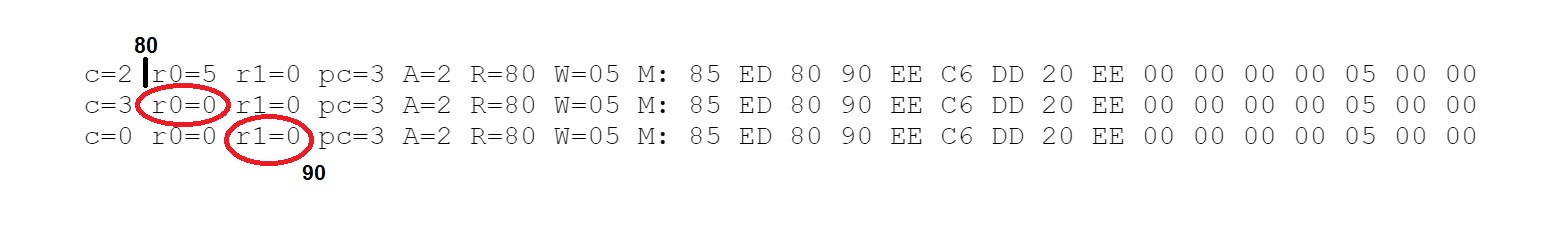
\includegraphics[width=1\linewidth]{graphics/log2}
	\end{figure}
	
	
	\subsection{Wyczyścić zawartość komórki o adresie 14, wpisując do niej 0.}
	
	\begin{table}[!ht]
		\centering
		\begin{tabular}{l|l|l|l}
		Opis                                                                  & OPCODE & MNEMONIC   & BYTE CODE \\ \hline
		wpisuje liczbę z rejestru R0 do komórki o adresie 14 & EE     & STR 0, 0xE & 11101110  \\
		\end{tabular}
	\end{table}
	Rezultat:
	
	\begin{figure}[!ht]
		\centering
		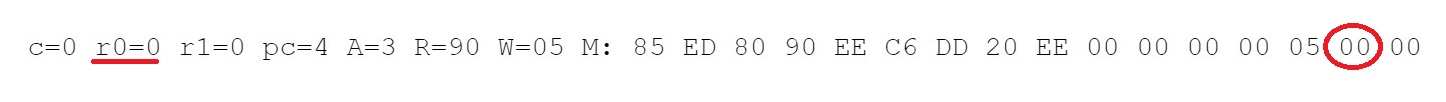
\includegraphics[width=1\linewidth]{graphics/log3}
	\end{figure}
	
	\newpage
	\subsection{Do rejestru R0 wpisać liczbę 0x6}
	
	\begin{table}[!ht]
		\centering
		\begin{tabular}{l|l|l|l}
	Opis                               & OPCODE & MNEMONIC & BYTE CODE \\ \hline
	wpisuje liczbę 0x6 do rejestru R0  & 86     & MOV 0x6  & 1000 0110 \\
	\end{tabular}
	\end{table}
	Rezultat:
	
	\begin{figure}[!ht]
		\centering
		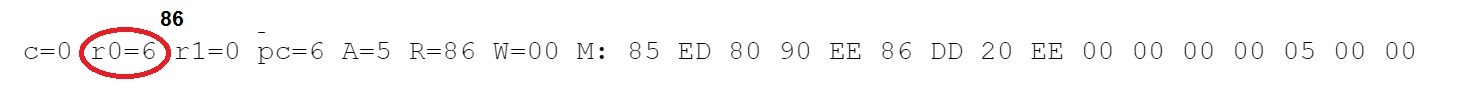
\includegraphics[width=1\linewidth]{graphics/log4}
	\end{figure}
	
	
	\subsection{Do rejestru R0 dodać wartość z pamięci pod adresem 13.}
	
	\begin{table}[!ht]
		\centering
		\begin{tabular}{l|l|l|l}
		Opis                               & OPCODE & MNEMONIC   & BYTE CODE \\ \hline
		do R1 wpisz wartość z adresu 13    & DD     & LDR 1, 0xD & 11011101  \\
		do R0 zapisz wynik R0+R1        & 20     & ADD R0, R1 & 0010 0000
		\end{tabular}
	\end{table}
	Rezultat:
	
	\begin{figure}[!ht]
		\centering
		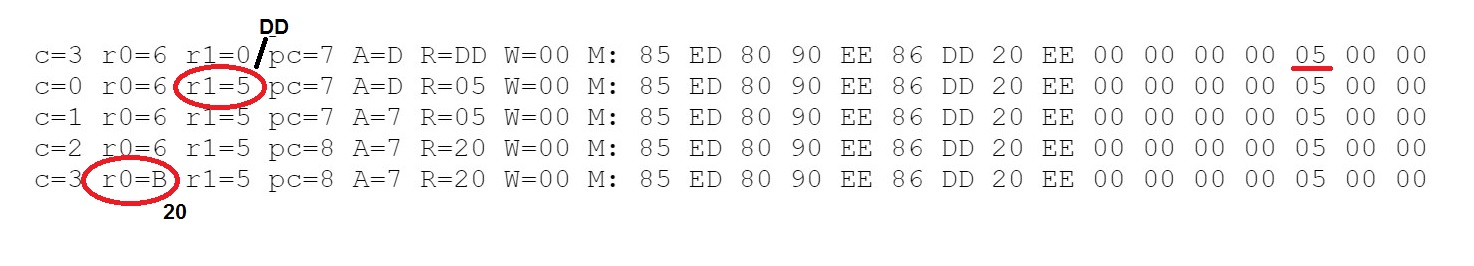
\includegraphics[width=1\linewidth]{graphics/log5}
	\end{figure}
	
	\subsection{Umieścić wartość rejestru R0 w pamięci w komórce o adresie 14}
	
	\begin{table}[!ht]
		\centering
		\begin{tabular}{l|l|l|l}
		Opis                            & OPCODE & MNEMONIC   & BYTE CODE \\ \hline
		zawartość R0 wpisz do adresu 14 & EE     & STR 0, 0xE & 1110 1110
		\end{tabular}
	\end{table}
	Rezultat:
	
	\begin{figure}[!ht]
		\centering
		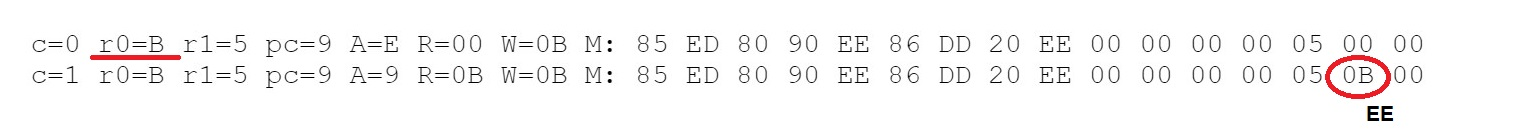
\includegraphics[width=1\linewidth]{graphics/log6}
	\end{figure}
	\newpage
	\subsection{Zapętlić wykonywanie programu.}
	
	\begin{table}[!ht]
		\centering
		\begin{tabular}{l|l|l|l}
		Opis                 & OPCODE & MNEMONIC & BYTE CODE \\ \hline
		skok do adresu nr. 0 & 0      & JMP 0x0  & 00000000 
		\end{tabular}
		\end{table}
	Rezultat:
	
	\begin{figure}[!ht]
		\centering
		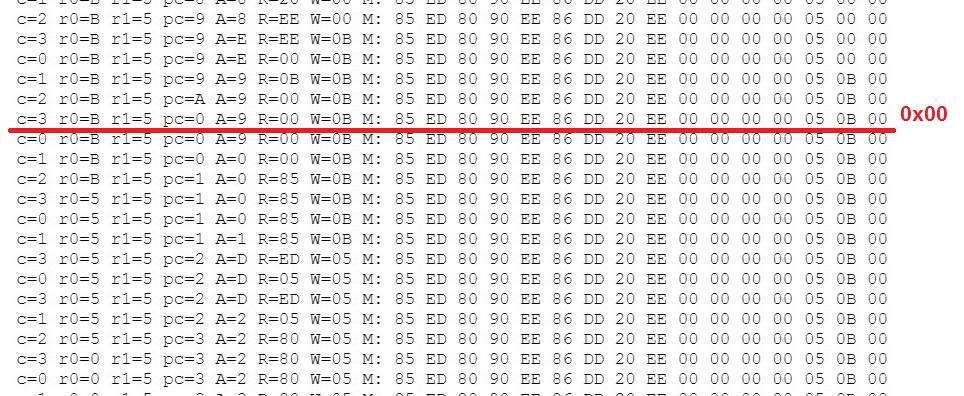
\includegraphics[width=1\linewidth]{graphics/log7}
	\end{figure}
	
	
		\newpage
	
	\section{Utworzenie nowej instrukcji mikroprocesora.}
	W pliku \texttt{cpu.v} w odpowiednim miejscu uzupełniliśmy kod o żądane instrukcje.
	\subsection{Do rejestru R1 zapisz wynik dodawania wartości z rejestrów Ro i R1.}
	\begin{figure}[!ht]
		\centering
		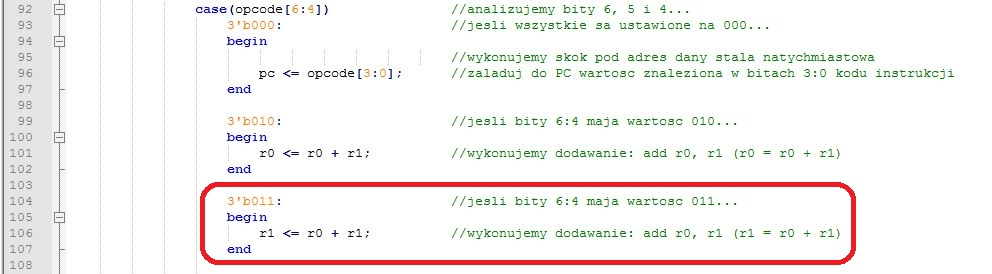
\includegraphics[width=1\linewidth]{graphics/code1}
	\end{figure}

	\subsection{Na rejestrach R0 i R1 zapisz (8bitowy) wynik mnożenia wartości z rejestrów R0 i R1}
	\begin{figure}[!ht]
		\centering
		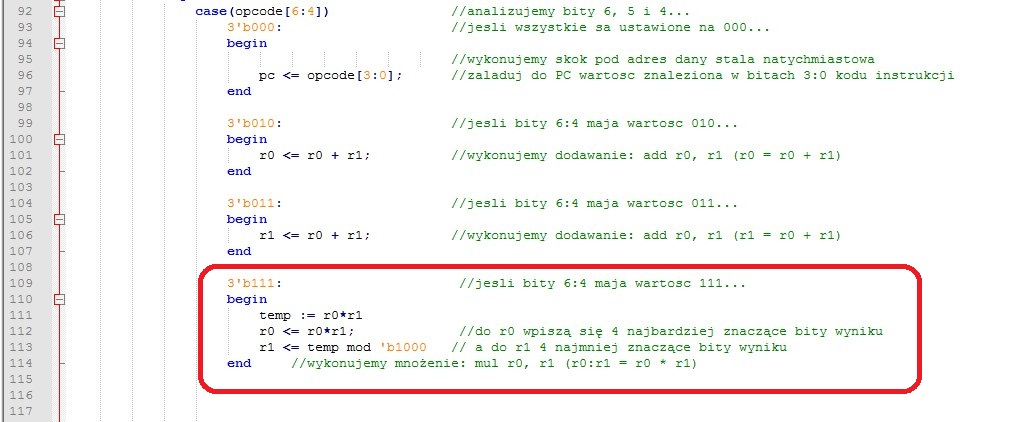
\includegraphics[width=1\linewidth]{graphics/code2}
	\end{figure}
	\section{Wnioski.}
	Wykonanie laboratorium 1 pozwoliło nam zapoznać się z podstawami programowania mikroprocesorów, w szczególności tych zrealizowanych w architekturze von Neumanna, oraz z obsługą płytek logiki programowalnej na przykładzie Digilent ZYBO.
	
\end{document}
	
	
